\section{State Space Complexity Derivation}
\label{sec:state-space-derivation}

This appendix derives combinatorial upper bounds on Pokémon team configuration and battle state spaces for Gen 1 OU, Gen 9 OU, and Gen 9 VGC.
We clearly distinguish \emph{exact} quantities (marked \textbf{E}), \emph{exact upper bounds} (marked \textbf{E upper bound}), and \emph{approximations} (marked \textbf{A}), and justify every choice.
Moves unavailable in Generation~9 (\texttt{isNonstandard:\ "Past"} in the Pok\'emon Showdown source) are excluded from the Gen~9 derivations.
All arithmetic has been verified programmatically.

% ─────────────────────────────────────────────────────────────────────────────
\subsection{EV Spread Counting}
\label{sec:ev-derivation}

\textbf{Setup.}
Each Pokémon distributes Effort Values (EVs) across 6 stats.
EVs only affect the stat formula in multiples of 4, so we count in units of 4.
Let $x_i \in \mathbb{Z}_{\geq 0}$ be the number of 4-EV units allocated to stat $i$.
The constraints are:
\begin{equation}
    \sum_{i=1}^{6} x_i \leq 127, \qquad 0 \leq x_i \leq 63.
    \label{eq:ev-constraint}
\end{equation}
The upper bounds reflect the per-stat cap of $252\,\text{EV} = 63 \times 4$ and the total budget of $508\,\text{EV} = 127 \times 4$.

\textbf{Exact count via inclusion-exclusion.}
Introduce slack variable $x_7 \geq 0$ so that $\sum_{i=1}^{7} x_i = 127$.
Stars-and-bars without the per-stat cap gives $\binom{133}{6} = 6{,}856{,}577{,}728$.
Applying inclusion-exclusion on $x_i \geq 64$ (substitute $y_i = x_i - 64$, remaining sum $= 63$) gives $\binom{69}{6} = 119{,}877{,}472$ per capped stat.
Two simultaneously capped stats would require total $\geq 128 > 127$, so higher-order terms vanish.

\begin{equation}
    \boxed{|\mathcal{E}| = \binom{133}{6} - 6\binom{69}{6} = 6{,}856{,}577{,}728 - 719{,}264{,}832 = 6{,}137{,}312{,}896.}
    \label{eq:ev-exact}
\end{equation}
\textbf{(E)} All arithmetic exact; no approximation.

% ─────────────────────────────────────────────────────────────────────────────
\subsection{Generation 9 Team Configuration Space}
\label{sec:gen9-derivation}

This bound applies to both Gen 9 OU and Gen 9 VGC, which draw from the same Pokémon pool.

\paragraph{Species \textbf{(E)}.}
\texttt{pokedex.ts} contains 1{,}329 standard entries for Generation 9: 1{,}025 base Pokémon (National Dex \#1--1025) plus 304 alternate formes.
Under Species Clause (no duplicates, unordered team of 6):
\begin{equation}
    \binom{1329}{6} = 7{,}566{,}741{,}017{,}135{,}560 \approx 7.57 \times 10^{15}.
\end{equation}

\paragraph{Movesets \textbf{(E upper bound)}.}
Mew has the largest movepool in Generation 9: exactly \textbf{375 moves}.
Using Mew's pool as the upper bound for all 6 team members:
\begin{equation}
    \binom{375}{4}^6 = 810{,}855{,}375^6 \approx 2.84 \times 10^{53}.
\end{equation}

\paragraph{Abilities \textbf{(E upper bound)}.}
Maximum 3 abilities per species (two standard plus one Hidden Ability):
\begin{equation}
    3^6 = 729.
\end{equation}

\paragraph{Individual Values \textbf{(E)}.}
Each stat has an IV in $\{0,\ldots,31\}$:
\begin{equation}
    \bigl(32^6\bigr)^6 = 32^{36} = 2^{180} \approx 1.53 \times 10^{54}.
\end{equation}

\paragraph{Effort Values \textbf{(E)}.}
Using the exact count from Section~\ref{sec:ev-derivation}:
\begin{equation}
    |\mathcal{E}|^6 = 6{,}137{,}312{,}896^6 \approx 5.34 \times 10^{58}.
\end{equation}

\paragraph{Natures \textbf{(E)}.}
25 natures exist, but 5 are neutral (all producing identical stat modifiers in battle), yielding $20 + 1 = 21$ functionally distinct natures:
\begin{equation}
    21^6 = 85{,}766{,}121.
\end{equation}

\paragraph{Held Items \textbf{(E)}.}
Generation 9 contains 248 standard held items:
\begin{equation}
    248^6 = 232{,}653{,}764{,}952{,}064 \approx 2.33 \times 10^{14}.
\end{equation}

\paragraph{Terastallization \textbf{(E)}.}
Each Pokémon may Terastallize into any of 19 types (the 18 standard types plus Stellar):
\begin{equation}
    19^6 = 47{,}045{,}881.
\end{equation}

\paragraph{Gen 9 team space.}
\begin{align}
    \mathcal{T}_{\text{Gen9}}
    &\approx \underbrace{7.57 \times 10^{15}}_{\text{species}} \times
       \underbrace{2.84 \times 10^{53}}_{\text{moves}} \times
       \underbrace{7.29 \times 10^{2}}_{\text{abilities}} \times
       \underbrace{1.53 \times 10^{54}}_{\text{IVs}} \times \notag \\
    &\quad \underbrace{5.34 \times 10^{58}}_{\text{EVs}} \times
       \underbrace{8.58 \times 10^{7}}_{\text{natures}} \times
       \underbrace{2.33 \times 10^{14}}_{\text{items}} \times
       \underbrace{4.70 \times 10^{7}}_{\text{Tera}} \notag \\
    &\approx \boxed{10^{215}}.
    \label{eq:gen9-total}
\end{align}
The moveset factor is an upper bound (using Mew's movepool for all species); all other factors are exact. The only approximation is the final $\log_{10}$ rounding.

% ─────────────────────────────────────────────────────────────────────────────
\subsection{Generation 1 OU (RBY) Team Configuration Space}
\label{sec:gen1-derivation}

Gen 1 lacks abilities, held items, natures, and Terastallization, but uses distinct mechanics for stats.

\paragraph{Species \textbf{(E)}.}
\begin{equation}
    \binom{151}{6} = 14{,}888{,}600{,}755 \approx 1.49 \times 10^{10}.
\end{equation}

\paragraph{Movesets \textbf{(E)}.}
Generation 1 contains 164 standard battle moves.
Mew can learn all of them via TMs/HMs; using the full 164-move pool for all 6 Pokémon:
\begin{equation}
    \binom{164}{4}^6 = 29{,}051{,}001^6 \approx 6.01 \times 10^{44}.
\end{equation}

\paragraph{Determinant Values (DVs) \textbf{(E)}.}
Attack, Defense, Speed, and Special DVs are each in $\{0,\ldots,15\}$; HP DV is determined by the others.
In competitive Gen~1 play, Defense, Speed, and Special DVs are always set to 15 (their maximum), as there is no strategic reason not to maximize them. The sole exception is Attack DV, which is sometimes set to 0 on special attackers to minimize self-damage from Confusion. Thus Attack DV $\in \{0, 15\}$ (2 values) and all other DVs are fixed, giving 2 choices per Pok\'emon:
\begin{equation}
    2^{6} = 64.
\end{equation}

\paragraph{Stat Experience \textbf{(E)}.}
Each stat has Stat Experience in $\{0,\ldots,65535\}$ (unsigned 16-bit integer), but in competitive Gen~1 play all Stat Experience values are always maxed at 65535 via full EV training---there is no strategic reason to leave any stat below maximum. This factor therefore collapses to 1 and does not contribute to the team space.

\paragraph{Gen 1 team space.}
\begin{align}
    \mathcal{T}_{\text{Gen1}}
    &= \underbrace{\binom{151}{6}}_{\mathbf{E}} \times
       \underbrace{\binom{164}{4}^6}_{\mathbf{E}} \times
       \underbrace{2^{6}}_{\mathbf{E}}
    \approx 1.49 \times 10^{10}
       \times 6.01 \times 10^{44}
       \times 64
    \approx \boxed{10^{57}}.
    \label{eq:gen1-total}
\end{align}

% ─────────────────────────────────────────────────────────────────────────────
\subsection{Battle State Spaces}
\label{sec:battle-state}

\paragraph{Common components.}

\emph{HP \textbf{(A)}.}
Current HP is an integer from 0 to maximum; we approximate with a representative $\text{max-HP} = 300$, giving 301 states (0--300) per Pok\'emon:
\begin{equation}
    301^{12} \approx 5.53 \times 10^{29}. \quad \mathbf{(A)}
\end{equation}
This is the only approximation in the derivation: actual max HP is determined by species, IVs, and EVs (already counted in the team space) and ranges from 1 (Shedinja) to $\sim$714 (Blissey). The representative value of 300 falls within the typical competitive range and does not materially affect the order-of-magnitude estimate.

\emph{Gen 9 field conditions \textbf{(E)}.}
\begin{align*}
    \text{Weather:} &\quad 1 + 4 \times 8 + 3 = 36 \text{ states} \\
                    &\qquad \text{(None; Sun/Rain/Sand/Snow with 1--8 turns; Harsh Sun/Heavy Rain/Strong Winds).} \\
    \text{Terrain:} &\quad 1 + 4 \times 8 = 33 \text{ states (None; Electric/Grassy/Misty/Psychic with 1--8 turns).}
\end{align*}

\emph{Side conditions \textbf{(E upper bound)}.}
Per-side conditions, each independent:
\begin{align*}
    \text{Hazards:} &\quad 2 \times 4 \times 3 \times 2 = 48 \text{ states} \\
                    &\qquad \text{(Stealth Rock on/off, Spikes 0--3, Toxic Spikes 0--2, Sticky Web on/off).} \\
    \text{Screens:} &\quad 9^3 = 729 \text{ states (Reflect/Light Screen/Aurora Veil each 0--8 turns).} \\
    \text{Tailwind:} &\quad 5 \text{ states (off or 1--4 turns).} \\
    \text{Safeguard:} &\quad 6 \text{ states (off or 1--5 turns).} \\
    \text{Mist:} &\quad 6 \text{ states (off or 1--5 turns).}
\end{align*}
Per-side total: $48 \times 729 \times 5 \times 6 \times 6 = 6{,}298{,}560$. Both sides: $6{,}298{,}560^2 \approx 10^{13.6}$.

\emph{Terastallization state \textbf{(E)}.}
Each player may Tera at most once per battle; state $=$ (whether Tera used) $\times$ (which of 6 Pokémon Tera'd, if applicable):
\begin{equation}
    (1 + 6)^2 = 49. \quad \mathbf{(E)}
\end{equation}

\emph{Pseudo-weather \textbf{(E)}.}
Turn-counted field-level volatile conditions:
\begin{align*}
    \text{Trick Room:} &\quad 6 \text{ states (off; 1--5 turns remaining).} \\
    \text{Gravity:} &\quad 6 \text{ states.} \\
    \text{Magic Room:} &\quad 6 \text{ states.} \\
    \text{Wonder Room:} &\quad 6 \text{ states.} \\
    \text{Fairy Lock:} &\quad 3 \text{ states (off; 1--2 turns remaining).}
\end{align*}
\begin{equation}
    \mathcal{P}_{\text{Gen9}} = 6^4 \times 3 = 3{,}888. \quad \mathbf{(E)}
\end{equation}

\emph{Slot conditions \textbf{(E)}.}
Conditions tied to a battlefield position (slot), not to the Pok\'emon occupying it.
In singles, there are 2 slots (one per side):
\begin{align*}
    \text{Wish:} &\quad 2 \text{ (pending or not).} \\
    \text{Future Sight/Doom Desire:} &\quad 3 \text{ (off; 1 or 2 turns remaining).} \\
    \text{Healing Wish:} &\quad 2 \text{ (pending or not).}
\end{align*}
Per slot: $2 \times 3 \times 2 = 12$. Two slots: $12^2 = 144$.

\emph{Per-active volatile statuses \textbf{(E upper bound)}.}
Each active Pok\'emon may simultaneously carry multiple volatile conditions.
We systematically enumerate all volatiles from the Pok\'emon Showdown source code (\texttt{conditions.ts}, \texttt{moves.ts}, \texttt{abilities.ts}), grouping mutually exclusive states.

\textbf{Independent binary/counter volatiles} (can all coexist).
We restrict to moves available in Generation~9; moves marked \texttt{isNonstandard:\ "Past"} in the Showdown source are excluded.\footnote{Excluded Past moves: Rage, Nightmare, Embargo, Heal Block, Octolock, Telekinesis, Foresight, Miracle Eye, Snatch, Grudge, Magic Coat, Laser Focus, Bide. These could technically be invoked via Metronome, but we adopt the same competitive-play framing used elsewhere in this derivation.}
Confusion (5: off or 2--5 turns),
Attract (2),
Leech Seed (2),
Substitute (2),
Taunt (5: off or 1--4 turns),
Encore (4: off or 1--3 turns),
Disable (5: off or 1--4 turns),
Torment (2),
Perish Song (4: off or 1--3 counter),
Aqua Ring (2),
Ingrain (2),
Focus Energy (2),
Yawn (3: off or 1--2 turns),
Curse (2),
No Retreat (2),
Tar Shot (2),
Salt Cure (2),
Syrup Bomb (4: off or 1--3 turns),
Imprison (2),
Charge (2),
Minimize (2),
Defense Curl (2),
Stockpile (4: 0--3 layers),
Glaive Rush (2),
Gastro Acid (2),
Power Trick (2),
Transform (2),
Trapped (2: Mean Look/Block/Shadow Tag),
Throat Chop (3: off or 1--2 turns),
Lock-On/Mind Reader (2).
\begin{equation}
    \mathcal{V}_{\text{indep}} \approx 6.04 \times 10^{11}. \quad \text{(product of all 30 factors above)}
\end{equation}

\textbf{Mutually exclusive groups} (at most one state per group):

\emph{Move locks} (a Pok\'emon can be locked into at most one multi-turn move):
None (1), locked move/Outrage etc.\ (1--3 turns = 3), two-turn move/Fly/Dig (1), must recharge/Hyper Beam (1), Uproar (1--3 turns = 3), Rollout (1--5 hits = 5), Ice Ball (1--5 hits = 5) $= 1+3+1+1+3+5+5 = 19$ states.

\emph{Protection moves} (at most one per turn):
None (1) + Protect, Baneful Bunker, Burning Bulwark, King's Shield, Obstruct, Silk Trap, Spiky Shield, Endure (8 variants) $= 9$ states.

\emph{Grounding/levitation} (mutually exclusive):
None (1), Smack Down (1), Magnet Rise (1--5 turns = 5) $= 7$ states.

\emph{Ability-specific volatiles} (a Pok\'emon has exactly one ability, so at most one applies):
None (1), Flash Fire active (1), Unburden active (1), Slow Start (1--5 turns = 5), Protosynthesis active (1), Quark Drive active (1) $= 10$ states.

\emph{Self-applied one-turn effects} (only one move per turn):
None (1), Roost (1), Destiny Bond (1) $= 3$ states.

\emph{Type changes}:
Type override (Soak, etc.): None (1) + 18 types + typeless from Burn Up (1) $= 20$ states.
Type addition: None (1) + Grass from Forest's Curse (1) + Ghost from Trick-or-Treat (1) $= 3$ states.

\emph{Choice lock} (from Choice Band/Scarf/Specs):
None (1) + locked into move 1/2/3/4 (4) $= 5$ states. Independent of multi-turn move locks above.

\emph{Other per-active factors}:
Stall counter (2: consecutive protect tracking), partial trapping (8: off or 1--7 turns), flinch (2), Powder (2), Electrify (2).

Combining all groups per active Pok\'emon:
\begin{align}
    \mathcal{V}_{\text{Gen9}} &= \mathcal{V}_{\text{indep}} \times 19 \times 9 \times 5 \times 2 \times 20 \times 3 \times 8 \times 2 \times 7 \times 10 \times 3 \times 2 \times 2 \notag \\
    &\approx 8.33 \times 10^{20}; \quad \mathcal{V}_{\text{Gen9}}^2 \approx 10^{41.8}. \quad \mathbf{(E\text{ upper bound})}
\end{align}

\emph{Item and ability state changes \textbf{(E upper bound)}.}
Items may be consumed, knocked off, or swapped (Trick/Switcheroo): 3 states per Pok\'emon.
Abilities may be suppressed or changed (Gastro Acid, Skill Swap, Mummy): 2 states per Pok\'emon.
\begin{equation}
    3^{12} \times 2^{12} \approx 10^{9.3}.
\end{equation}

\emph{PP.}
We omit move PP from the state space count. In competitive play, PP depletion is strategically relevant only in niche stalling scenarios; the vast majority of games end well before any move runs out of PP. Including binary PP tracking ($2^{48} \approx 10^{14.4}$) would increase all totals by $\sim$14 orders of magnitude but would not meaningfully reflect the strategic state of typical competitive battles.


\emph{Non-volatile status conditions \textbf{(E upper bound)}.}
Each Pok\'emon carries at most one non-volatile status, which persists through switches.
In Gen~9 the possible states per Pok\'emon are:
Healthy~(1), Burn~(1), Freeze~(1), Paralysis~(1), Poison~(1), Toxic~(1), Sleep with turn counter 1--3~(3):
\begin{equation}
    \mathcal{C}_{\text{Gen9}} = 9^{12} \approx 2.82 \times 10^{11}. \quad \mathbf{(E\text{ upper bound})}
\end{equation}

% ─────────────────────────────────────────────────────────────────────────────
\paragraph{Gen 9 OU (singles).}

\emph{Active Pokémon \textbf{(E)}.}
One of 6 active per side: $6 \times 6 = 36$ arrangements.

\emph{Stat stages \textbf{(E)}.}
2 active Pokémon × 7 modifiable stats (Atk, Def, SpA, SpD, Spe, Acc, Eva), each $\in [-6,+6]$ (13 values):
\begin{equation}
    13^{14} \approx 3.94 \times 10^{15}.
\end{equation}

\begin{align}
    \text{Gen 9 OU battle state}
    &= \mathcal{T}_{\text{Gen9}}^2 \times 36 \times 301^{12} \times 13^{14} \times \mathcal{C}_{\text{Gen9}} \notag \\
    &\quad \times 36 \times 33 \times 6{,}298{,}560^2 \times 49 \times \mathcal{P}_{\text{Gen9}} \times 12^2 \notag \\
    &\quad \times \mathcal{V}_{\text{Gen9}}^{2} \times 3^{12} \times 2^{12} \notag \\
    &\approx 10^{430} \times 10^{1.6} \times 10^{29.7} \times 10^{15.6} \times 10^{11.5} \notag \\
    &\quad \times 10^{1.6} \times 10^{1.5} \times 10^{13.6} \times 10^{1.7} \times 10^{3.6} \times 10^{2.2} \notag \\
    &\quad \times 10^{41.8} \times 10^{5.7} \times 10^{3.6} \notag \\
    &\approx \boxed{10^{564}}.
    \label{eq:gen9-ou-battle}
\end{align}

% ─────────────────────────────────────────────────────────────────────────────
\paragraph{Gen 9 VGC (doubles).}

VGC is a doubles format: each player has \emph{two} Pokémon active simultaneously, with position (left/right) mattering for targeting.
Each player also chooses which 4 of 6 Pokémon to bring during team preview (hidden from opponent).

\emph{Team preview \textbf{(E)}.}
$\binom{6}{4}^2 = 15^2 = 225$ joint selections.

\emph{Active positions \textbf{(E)}.}
Ordered pairs of active Pokémon from the 4 brought per side (left/right positions distinct): $P(4,2)^2 = (4 \times 3)^2 = 144$.

\emph{Stat stages \textbf{(E)}.}
4 active Pokémon × 7 modifiable stats:
\begin{equation}
    13^{28} \approx 1.55 \times 10^{31}.
\end{equation}


Since only 4 Pok\'emon per side participate in each VGC battle, HP is counted over 8 (not 12), non-volatile status over 8, and Terastallization over the 4 brought per side: $(1+4)^2 = 25$.

VGC adds several doubles-specific side conditions not present in singles:
Fire/Water/Grass Pledge field effects (5 states each, turn-counted),
Quick Guard (2), Wide Guard (2), Crafty Shield (2), Mat Block (2).
The per-side total becomes $6{,}298{,}560 \times 5^3 \times 2^4 = 12{,}597{,}120{,}000$, so both sides: $\sim 10^{20.2}$.

Per-active volatiles gain doubles-specific additions:
Helping Hand (2), redirection---Follow Me/Rage Powder/Spotlight (mutually exclusive, 4 states), Dragon Cheer (2), Ally Switch (2).
Slot conditions have 4 slots (2 per side) instead of 2: $12^4 = 20{,}736$.

\begin{align}
    \text{Gen 9 VGC battle state}
    &= \mathcal{T}_{\text{Gen9}}^2 \times 225 \times 144 \times 301^{8} \times 13^{28} \notag \\
    &\quad \times 9^{8} \times 36 \times 33 \times \text{SC}_{\text{VGC}}^2 \times 25 \times \mathcal{P}_{\text{Gen9}} \times 12^4 \notag \\
    &\quad \times \mathcal{V}_{\text{VGC}}^{4} \times 3^{8} \times 2^{8} \notag \\
    &\approx 10^{430} \times 10^{2.4} \times 10^{2.2} \times 10^{19.8} \times 10^{31.2} \notag \\
    &\quad \times 10^{7.6} \times 10^{1.6} \times 10^{1.5} \times 10^{20.2} \times 10^{1.4} \times 10^{3.6} \times 10^{4.3} \notag \\
    &\quad \times 10^{89.7} \times 10^{3.8} \times 10^{2.4} \notag \\
    &\approx \boxed{10^{622}}.
    \label{eq:gen9-vgc-battle}
\end{align}

% ─────────────────────────────────────────────────────────────────────────────
\paragraph{Gen 1 OU (singles).}

Gen 1 has no weather, terrain, entry hazards, or screens.
Status conditions per Pokémon: Healthy + BRN + FRZ + PAR + PSN + bad PSN (turn counter 1--15) + SLP (turn counter 1--7) $= 1+1+1+1+1+15+7 = 27$ states\footnote{Toxic poison in Gen 1 deals $\lfloor N/16 \rfloor \times \text{max-HP}$ damage on turn $N$, so the counter 1--15 produces 15 distinct in-battle trajectories.}; for 12 Pokémon: $27^{12} \approx 10^{17.2}$ \textbf{(E)}.
Stat stages: 2 active Pokémon × 6 stats (Attack, Defense, Special, Speed, Evasion, Accuracy), each $\in [-6,+6]$: $13^{12} \approx 10^{13.4}$ \textbf{(E)}.

\emph{Per-active volatile statuses \textbf{(E upper bound)}.}
Volatile conditions that apply only to active Pok\'emon (cleared on switch).
In Gen~1, Reflect and Light Screen are per-Pok\'emon volatiles rather than field-wide screens.
Per active Pok\'emon:

\textbf{Independent:}
Confusion (5: none or 1--4 turns),
Leech Seed (2),
Substitute (2),
Focus Energy (2),
Disable (29: off, or one of 4 moves $\times$ 1--7 turns),
Reflect (2),
Light Screen (2),
Mist (2),
Minimize (2),
Transform (2),
Rage (2).

\textbf{Mutually exclusive move locks:}
None (1), Thrash lock (1--3 turns = 3), two-turn move/Fly/Dig (1), must recharge (1), Bide (1--2 turns = 2), partial trapping lock (1--4 turns = 4) $= 12$ states.

\textbf{Other per-active:}
Partial trapping (defender side, 5: off or 1--4 turns),
residual damage counter (16: 0--15, tracks toxic/trap damage),
flinch (2).

\begin{equation}
    \mathcal{V}_{\text{Gen1}} = (5 \times 2^7 \times 29 \times 2^2) \times 12 \times 5 \times 16 \times 2 = 142{,}540{,}800 \approx 10^{8.2}.
\end{equation}
\begin{equation}
    \mathcal{V}_{\text{Gen1}}^{2} \approx 10^{16.3}. \quad \mathbf{(E\text{ upper bound})}
\end{equation}

\begin{align}
    \text{Gen 1 OU battle state}
    &= \mathcal{T}_{\text{Gen1}}^2
       \times 36
       \times 301^{12}
       \times 13^{12}
       \times 27^{12}
       \times \mathcal{V}_{\text{Gen1}}^{2} \notag \\
    &\approx 10^{114}
       \times 10^{1.6}
       \times 10^{29.7}
       \times 10^{13.4}
       \times 10^{17.2}
       \times 10^{16.3}
    \approx \boxed{10^{192}}.
    \label{eq:gen1-battle}
\end{align}

% ─────────────────────────────────────────────────────────────────────────────
\subsection{Summary}

\begin{table}[H]
\centering
\setlength{\tabcolsep}{8pt}
\caption{
State space complexity across Pokémon formats and classical games.
All Pokémon components are exact \textbf{(E)} except HP values (marked \textbf{A}); status conditions and volatile statuses are exact upper bounds.
Team space values are upper bounds.
Battle state includes item consumption/knockout state and ability suppression/swap state; PP is omitted as it is rarely strategic in competitive play (see text).
Volatile statuses are enumerated from the Pok\'emon Showdown source code with mutual exclusion groups (protect variants, move locks, grounding/levitation, ability-specific volatiles, self-applied one-turn effects) properly handled.
Gen 9 OU and VGC share the same team pool; VGC's larger battle state reflects 4 simultaneously active Pokémon (vs.\ 2 in singles), hidden team preview selection, and doubles-specific side conditions and volatiles.
}
\label{tab:state-space-comparison}
\resizebox{\textwidth}{!}{%
\begin{tabular}{@{}cccc@{}}
\toprule
\textbf{Format} & \textbf{Team Space (1 player)} & \textbf{Battle State Space} & \textbf{Notes} \\
\midrule
Gen 1 OU (RBY)   & $\sim 10^{57}$ & $\sim 10^{192}$ & Singles; no items/abilities/natures; competitive DV constraints \\
Gen 9 OU         & $\sim 10^{215}$ & $\sim 10^{564}$ & Singles; Terastallization \\
Gen 9 VGC        & $\sim 10^{215}$ & $\sim 10^{622}$ & Doubles; bring 4 of 6; team preview \\
\midrule
Chess            & ---             & $\sim 10^{47}$  & --- \\
Go               & ---             & $\sim 10^{170}$ & --- \\
\bottomrule
\end{tabular}%
}
\end{table}


\subsection{Team Space in Human Metagame}

The combinatorial space of Pokémon teams is vast when enumerating all \textit{legal} combinations of species, moves, items, abilities, and stat spreads (Table \ref{tab:state-space-comparison}). In practice, however, the effective space considered by competitive players is considerably smaller. Many options are dominated by clearly superior alternatives. For example, two moves may share the same type and role, but if one is less powerful and reliable, there is no competitive reason to justify its selection. Similar dominance relationships apply to items, abilities, and stat spreads. Table \ref{tab:gen1-vs-gen9-team-metrics} estimates this state-space reduction by restricting to options that Showdown players above a \textasciitilde median skill rating select in at least 1\% of battles. A second factor is metagame convergence. Even among viable options, competitive play concentrates around successful team archetypes as players adapt to one another. Figure \ref{fig:team_complexity_usage_stats} provides an example: a small fraction of available Pokémon account for the majority of human choices. Nevertheless, the number of competitively viable combinations is exceptionally large, and team design in competitive Pokémon remains a daunting optimization problem.


\begin{table}[h!]
\centering
\caption{\textbf{Effective team space on Showdown Gen~1 OU and Gen~9 OU ladders.}
Derived from public usage statistics (2014--2025, Glicko-1~$\geq$1500).
Only options appearing on at least 1\% of teams (for species) or 1\% of
that species' sets (for moves, items, abilities, and EV/nature spreads)
are counted.}
\label{tab:gen1-vs-gen9-team-metrics}
\resizebox{0.5\textwidth}{!}{%
\begin{tabular}{@{}lcc@{}}
\toprule
\textbf{} & \textbf{Gen 1 OU} & \textbf{Gen 9 OU} \\
\midrule
Species in pool & 45 & 117 \\
\midrule
Avg.\ moves per species & 13.0 & 14.0 \\
Avg.\ items per species & --- & 6.6 \\
Avg.\ abilities per species & --- & 1.7 \\
Avg.\ EV/nature spreads per species & --- & 7.8 \\
\midrule
Team state space ($\log_{10}$) & 23.5 & 37.8 \\
\bottomrule
\end{tabular}%
}
\end{table}


\begin{figure}[h!]
    \centering
    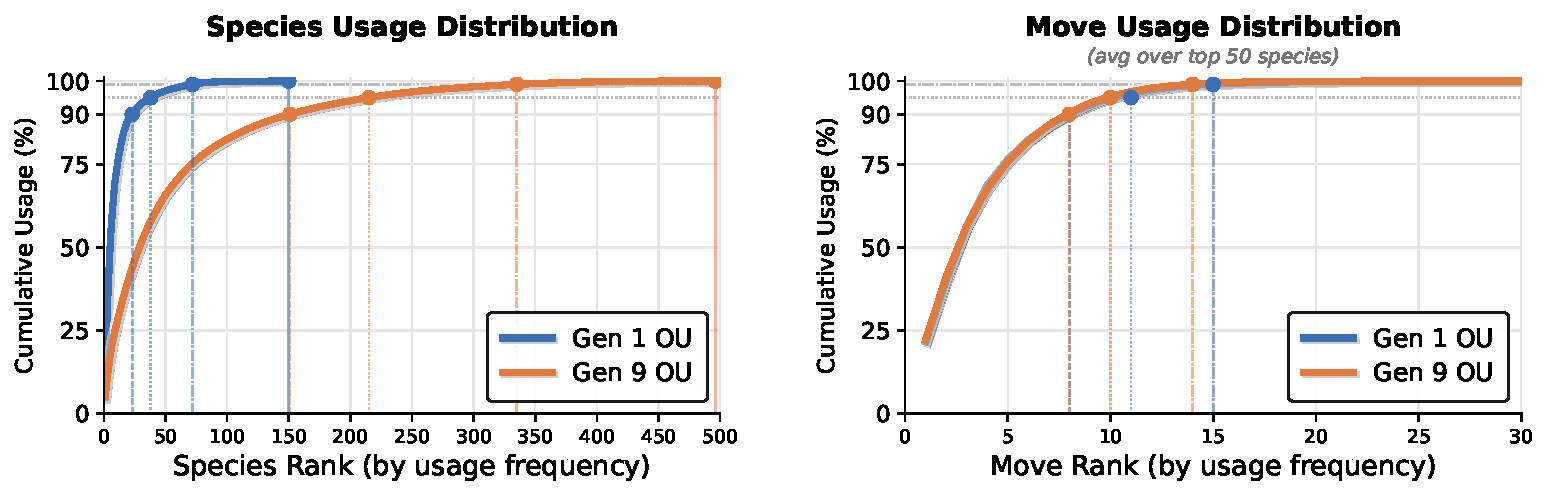
\includegraphics[width=0.9\linewidth]{figures/team_complexity_usage_stats.pdf}
    \caption{\textbf{Empirical usage distributions in Gen~1 OU and Gen~9 OU}. Derived from Smogon usage statistics (2014--2025,
rank~$\geq$1500).
\textbf{Left:} cumulative species usage---the fraction of all team-slot
appearances accounted for by the top-$k$ most-used species.
\textbf{Right:} cumulative move usage per species, averaged over the
top-50 species in each format.}
    \label{fig:team_complexity_usage_stats}
\end{figure}